\chapter{Codebase: Basket Panel}

The basket is a client side construct, in the sense that there is no
model or data to represent a basket in the server side.  It forms a 
station to which to push the relevant plottables or containers.

This contents of this station act as a selection.  Using the
application, one can plot the selection 'PlotBasket' or attach
metadata to each of the chosen objects, etc.

\section{Description}

Like the list-panel, the basket is also a fixed width table of objects
with each item having a set of action buttons configurable while
defining the list.  The Basket also has some operative buttons.

\begin{description}
  \item[clear] \hfill \\
  Clears the contents of the basket.

  \item[save \emph{Not implemented}] \hfill \\
  Saves the contents of the basket as a selection for the user.

  \item[load \emph{Not implemented}] \hfill \\
  Loads the contents of a selection on the server.  These selections
  are usually the result of a save operation on the server by the
  previous 'save' feature.

  \item[plot]
  Plots the contents of the basket into the plotting panel on the
  'plot' tab.

  \item[edit metadata]
  Attaches metadata to each of the basket's items.
\end{description}

\begin{figure}[h!t]
  \centering
  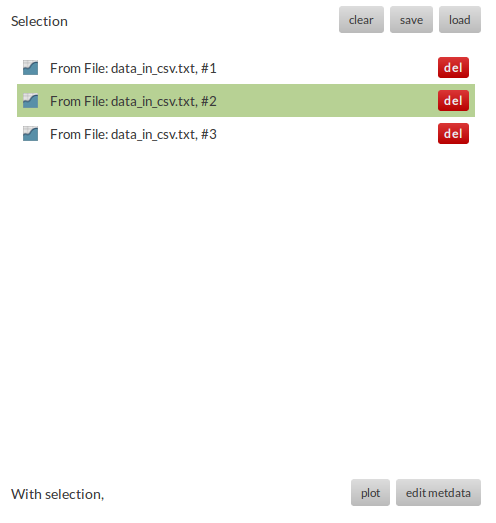
\includegraphics[width=\textwidth]{src/images/wdat-basket.png}
  \caption{ListPanel}
\end{figure}

\section{Methods}

There are a few methods exposed by the wdat.basket module.

\begin{enumerate}
  \item{wdat.basket.push()} \hfill \\
  Add item to the basket.

  \item{wdat.basket.clear()} \hfill \\
  Clears the basket.

  \item{wdat.basket.data()} \hfill \\
  Allows you to get/set the list of objects contained in the basket.
  Helpful for replacing the contents with an entirely different list.
  eg. In loading a selection from the server.

  \item{wdat.basket.del()} \hfill \\
  Allows deletion of single elements referred to by their unique ids.
\end{enumerate}
